\documentclass{article}

\usepackage[utf8]{inputenc}
\usepackage{amsmath}
\usepackage{amsfonts}
\usepackage{amssymb}
\usepackage{graphicx}
\usepackage[table,xcdraw]{xcolor}
\usepackage[hidelinks]{hyperref}
\usepackage{fontawesome5}
\usepackage{longtable}


\graphicspath{ {./images/} }

\renewcommand{\contentsname}{Indice}

\makeatletter
\newcommand*{\rom}[1]{\expandafter\@slowromancap\romannumeral #1@}
\makeatother

\usepackage[a4paper,top=2cm,bottom=2cm,left=2cm,right=2cm]{geometry}


\title{\textbf{\Huge Specifica dei Requisiti}}
\author{Edoardo Ghirardello, Giulio Cappelli, Elia Casotti \\ \\ Gruppo T42}
\date{2022}

\let\origthesubsection\thesubsection

\begin{document}

\maketitle

\clearpage
\tableofcontents
\clearpage

\section{Scopo del documento}
\begin{description}
    \item[] Questo documento riporta la specifica dei requisiti di sistema del sistema "Fen Festa", impiegando diversi tipologie di diagrammi UML quali:
        \begin{itemize}
            \item Diagramma dei Casi d'Uso (Use-Case Diagram)
            \item Diagramma di Contesto (Context Diagram)
            \item Diagramma dei Componenti (Component Diagram)
        \end{itemize}
\end{description}
\clearpage
\section{Requisiti Funzionali}
\begin{description}
    \item[] Nel seguente capitolo vengono riportati i Requisiti Funzionali (RF) del sistema utilizzando il linguaggio naturale e Use Case Diagram scritti in UML
\end{description}
\renewcommand\thesubsection{}
\subsection{RF1 Visualizzazione Eventi}
\subsection{RF2 Ricerca Eventi}
\subsection{RF3 Visualizzazione Descrizione Evento (Utente Non Registrato)}
\subsection{RF4 Visualizzazione Descrizione Evento (Utente Registrato)}
\begin{center}
    \item[] 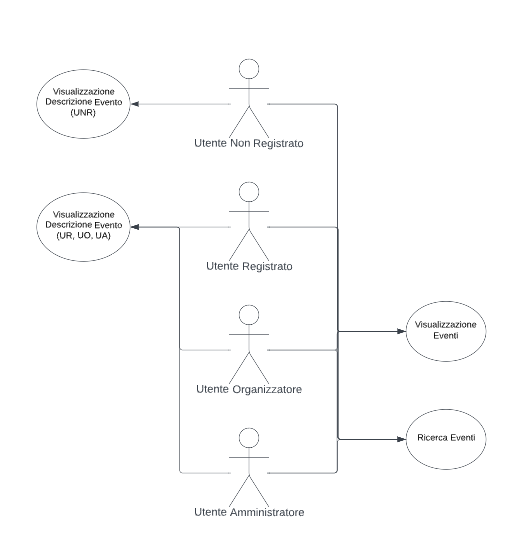
\includegraphics[scale=0.7]{UseCase_1.png}
\end{center}
\subsubsection*{Descrizione Use Case "Visualizzazione Eventi"}
\begin{description}
    \item[] Titolo: Visualizzazione Evento
    \item[] Riassunto: Questo Use Case descrive come avviene la visualizzazione di un evento
    \item[] Descrizione:
        \begin{enumerate}
            \item Gli utenti UNR, UR, UO o UA accedono alla pagina "Home" dove visualizzeranno la lista degli eventi
            \item Gli utenti sceglie il range temporale in cui filtrare gli eventi (Giorno, Settimana, Mese) tramite un selezionatore di data
            \item Il sistema poi mostrerà tutti gli eventi aventi la data o il range temporale selezionato
        \end{enumerate}
\end{description}
\subsubsection*{Descrizione Use Case "Ricerca Eventi"}
\begin{description}
    \item[] Titolo: Ricerca Eventi
    \item[] Riassunto: Questo Use Case descrive come avviene la ricerca di un evento
    \item[] Descrizione:
        \begin{enumerate}
            \item Gli utenti UNR, UR, UO o UA accedono alla pagina "Home" dove potranno cliccare sull'icona \faIcon{search}
            \item Una volta selezionata l'icona l'utente successivamente inserisce cosa ricercare (tag o nome dell'evento)
            \item Il sistema poi mostrerà tutti gli eventi aventi i tag o il nome inseriti
        \end{enumerate}
\end{description}
\subsubsection*{Descrizione Use Case "Visualizzazione Descrizione Evento"}
\begin{description}
    \item[] Titolo: Visualizzazione Descrizione Evento
    \item[] Riassunto: Questo Use Case descrive come avviene la visualizzazione delle informazioni riguardanti un evento
    \item[] Descrizione:
        \begin{enumerate}
            \item Gli utenti UNR, UR, UO o UA accede alla pagina "Home" dove visualizzeranno la lista degli eventi
            \item L'utente preme su un evento specifico
            \item Il sistema mostra l'evento nel suo intero mostrando:
                  \begin{itemize}
                      \item Nome
                      \item Immagine
                      \item Descrizione
                      \item Tag
                      \item Data e Ora
                      \item Luogo (Posizione/Indirizzo)
                      \item Numero partecipanti
                  \end{itemize}
            \item Poi in base a che tipo di utente è: UNR o UR/UO/UA il sistema mostra anche due tasti:
                  \begin{itemize}
                      \item Tasto "Partecipo"
                      \item Tasto "Salva Evento"
                  \end{itemize}
                  che permettono a UR, UO, UA di poter salvare l'evento nei preferiti (e ricevere una mail di notifica riguardane l'inizio dell'evento) e far sapere agli altri utenti che parteciperà all'evento in questione
        \end{enumerate}
\end{description}
\clearpage
\subsection{RF5 Creazione Evento}
\subsection{RF6 Modifica Evento}
\subsection{RF7 Eliminazione Evento}
\begin{center}
    \item[] 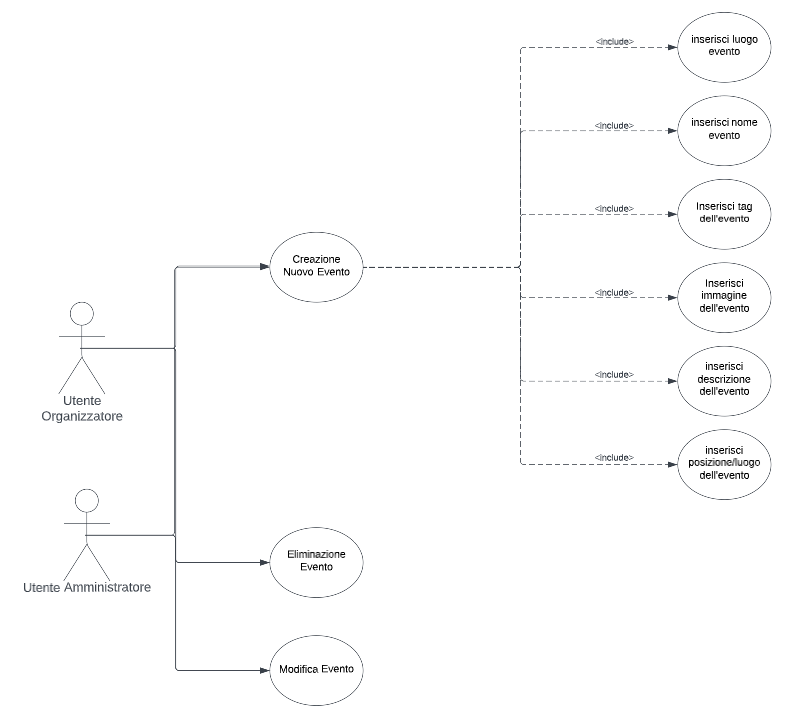
\includegraphics[scale=0.5]{UseCase_2.png}
\end{center}
\subsubsection*{Descrizione Use Case "Creazione Evento"}
\begin{description}
    \item[] Titolo: Creazione Evento
    \item[] Riassunto: Questo Use Case descrive come avviene la procedura di creazione di un evento
    \item[] Descrizione:
        \begin{enumerate}
            \item Gli utenti UO o UA accedono alla pagina "Home" dove potranno cliccare sull'icona \faIcon{pencil-alt}
            \item Una volta selezionata l'icona il sistema mostra un form in cui l'utente deve inserire nei campi i dati richiesti:
                  \begin{itemize}
                      \item Nome
                      \item Immagine
                      \item Descrizione
                      \item Tag
                      \item Data e Ora
                      \item Luogo (Posizione/Indirizzo)
                  \end{itemize}
            \item Una volta inseriti i dati il sistema controlla che tutti i campi siano stati compilati \hyperref[exc:5.1]{[exception 1]}
        \end{enumerate}
    \item[] Exceptions:
        \begin{description}
            \item[] \label{exc:5.1} [exception 1] Tutti i campi devono essere compilati
        \end{description}
\end{description}
\subsubsection*{Descrizione Use Case "Eliminazione Evento"}
\begin{description}
    \item[] Titolo: Eliminazione Evento
    \item[] Riassunto: Questo Use Case descrive come avviene la procedura di eliminazione di un evento
    \item[] Descrizione:
        \begin{enumerate}
            \item Gli utenti UO o UA accedono alla pagina "Home" dove potranno cliccare su un proprio evento
            \item Una volta selezionata l'evento, il sistema mostra all'utente la descrizione e i tasti modifica ed elimina
            \item Cliccando su modifica l'utente proprietario dell'evento accede a un form identico a quello della creazione evento, ma precompilato con i dati inseriti in fase di creazione. Può modificare ogni campo.
            \item Cliccando in basso su "elimina" l'utente proprietario dell'evento eliminerà l'evento
        \end{enumerate}
\end{description}
\subsubsection*{Descrizione Use Case "Modifica Evento"}
\begin{description}
    \item[] Titolo: Modifica Evento
    \item[] Riassunto: Questo Use Case descrive come avviene la procedura di modifica di un evento
    \item[] Descrizione:
        \begin{enumerate}
            \item Gli utenti UO o UA accedono alla pagina "Home" dove potranno cliccare su un proprio evento
            \item Una volta selezionata l'evento, il sistema mostra all'utente la descrizione e i tasti modifica ed elimina
            \item Cliccando su modifica l'utente proprietario dell'evento accede a un form identico a quello della creazione evento, ma precompilato con i dati inseriti in fase di creazione. Può modificare ogni campo.
            \item Cliccando in basso su "modifica" l'utente proprietario dell'evento salverà le modifiche apportate ai campi precedenti
        \end{enumerate}
\end{description}
\clearpage
\subsection{RF8 Login}
\subsection{RF9 Recupero Password}
\subsection{RF10 Creazione Account}
\subsection{RF11 Conferma Creazione Account}
\begin{center}
    \item[] 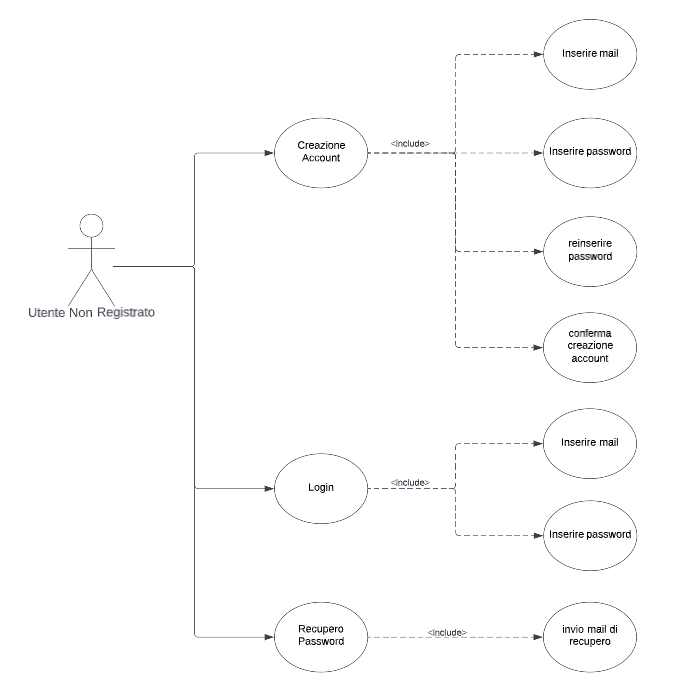
\includegraphics[scale=0.5]{UseCase_3.png}
\end{center}
\subsubsection*{Descrizione Use Case "Login"}
\begin{description}
    \item[] Titolo: Login
    \item[] Riassunto: Questo Use Case descrive come avviene la procedura di login
    \item[] Descrizione:
        \begin{enumerate}
            \item L'utente UNR una volta selezionata la pagina "Impostazioni" tramite l'icona \faIcon{cog} può selezionare il tasto "Login" per eseguire l'accesso
            \item Il sistema successivamente mostra all'utente il form di login dove richiede all'utente di inserire:
                  \begin{itemize}
                      \item Email
                      \item Password
                  \end{itemize}
            \item Una volta compilati i campi il sistema controlla che siano stati correttamente compilati \hyperref[exc:8.1]{[exception 1]}
        \end{enumerate}
    \item[] Exceptions:
        \begin{description}
            \item[] \label{exc:8.1} [exception 1] Tutti i campi devono essere compilati
        \end{description}
\end{description}
\clearpage
\subsubsection*{Descrizione Use Case "Recupero Password"}
\begin{description}
    \item[] Titolo: Recupero Password
    \item[] Riassunto: Questo Use Case descrive come avviene la procedura di recupero della password
    \item[] Descrizione:
        \begin{enumerate}
            \item L'utente UNR una volta selezionata la pagina "Impostazioni" tramite l'icona \faIcon{cog} dalla home può selezionare il tasto "Login" per eseguire l'accesso
            \item Se l'utente non riesce a effettuare il Login poiché non si ricorda la password la può reimpostare tramite il tasto "Reimposta Password"
            \item Il sistema successivamente mostra all'utente un campo dove inserire la propria mail \hyperref[exc:9.1]{[exception 1]}
            \item Una volta inserita la mail il sistema invierà tramite un sistema di invio mail una password temporanea che successivamente l'utente dovrà cambiare
        \end{enumerate}
    \item[] Exceptions:
        \begin{description}
            \item[] \label{exc:9.1} [exception 1] Tutti i campi devono essere compilati
        \end{description}
\end{description}
\subsubsection*{Descrizione Use Case "Creazione Account"}
\begin{description}
    \item[] Titolo: Creazione Account
    \item[] Riassunto: Questo Use Case descrive come avviene la procedura di creazione di un nuovo account
    \item[] Descrizione:
        \begin{enumerate}
            \item L'utente UNR una volta selezionata la pagina "Impostazioni" tramite l'icona \faIcon{cog} dalla home può selezionare il tasto "Crea Account" per creare un nuovo account
            \item Il sistema presenta all'utente un form in cui deve inserire:
                  \begin{itemize}
                      \item Email
                      \item Password
                      \item Conferma Password
                  \end{itemize}
            \item Una volta compilato il form il sistema controlla che i campi siano tutti compilati \hyperref[exc:10.1]{[exception 1]} e che "Conferma Password" deve essere uguale al campo "Password" \hyperref[exc:10.2]{[exception 2]}
            \item Il sistema una volta creato l'account invia tramite sistema di mail una conferma della creazione dell'account (RF11)
        \end{enumerate}
    \item[] Exceptions:
        \begin{description}
            \item[] \label{exc:10.1} [exception 1] Tutti i campi devono essere compilati
            \item[] \label{exc:10.2} [exception 1] Il campo "Conferma Password" deve essere uguale al campo "Password"
        \end{description}
\end{description}
\clearpage
\subsection{RF12 Modifica Profilo}
\subsection{RF14 Richiesta Upgrade a UO}
\begin{center}
    \item[] 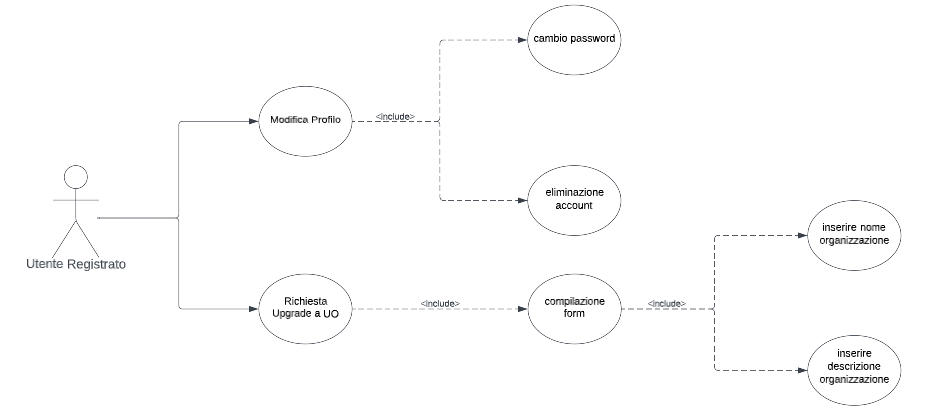
\includegraphics[scale=0.5]{UseCase_4.png}
\end{center}
\subsubsection*{Descrizione Use Case "Modifica Profilo"}
\begin{description}
    \item[] Titolo: Modifica Profilo
    \item[] Riassunto: Questo Use Case descrive come avviene la procedura di modifica del profilo
    \item[] Descrizione:
        \begin{enumerate}
            \item L'utente UR una volta selezionata la pagina "Impostazioni" tramite l'icona \faIcon{cog} dalla home può selezionare i tasti "Cambio Password" e "Eliminazione Account".
                  \begin{itemize}
                      \item Cambio Password: selezionando "Cambio Password" l'utente potrà inserire: nuova password, conferma nuova password \hyperref[exc:12.1]{[exception 1]}\hyperref[exc:12.2]{[exception 2]}
                      \item Eliminazione Account: selezionando "Eliminazione Account" l'utente potrà eliminare il proprio account. È necessario confermare cliccando su un pop-up
                  \end{itemize}
        \end{enumerate}
    \item[] Exceptions:
        \begin{description}
            \item[] \label{exc:12.1} [exception 1] Tutti i campi devono essere compilati
            \item[] \label{exc:12.2} [exception 2] Il campo "Conferma Password" deve essere uguale al campo "Password"
        \end{description}
\end{description}
\subsubsection*{Descrizione Use Case "Richiesta Upgrade a UO"}
\begin{description}
    \item[] Titolo: Richiesta Upgrade a UO
    \item[] Riassunto: Questo Use Case descrive come avviene la procedura di upgrade dell'utente da UR a UO
    \item[] Descrizione:
        \begin{enumerate}
            \item L'utente UR una volta selezionata la pagina "Impostazioni" tramite l'icona \faIcon{cog} dalla home può selezionare "Upgrade A Organizzatore"
            \item L'utente deve compilare un form contenente:
                  \begin{itemize}
                      \item nome organizzazione
                      \item descrizione organizzazione
                  \end{itemize}
                  \hyperref[exc:14.1]{[exception 1]}
            \item Il sistema manderà una mail agli admin per elaborare la richiesta (eventuali ulteriori messaggi effettuati all'esterno del sistema)
        \end{enumerate}
    \item[] Exceptions:
        \begin{description}
            \item[] \label{exc:14.1} [exception 1] Tutti i campi devono essere compilati
        \end{description}
\end{description}
\clearpage
\subsection{RF13 Modifica Profilo (UO)}
\begin{center}
    \item[] 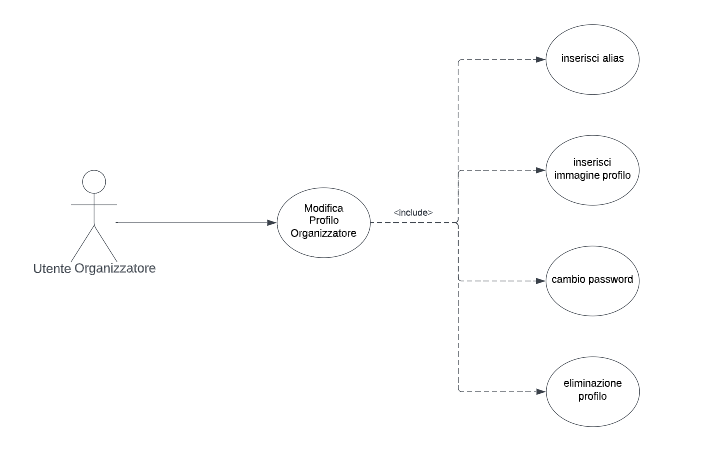
\includegraphics[scale=0.5]{UseCase_6.png}
\end{center}
\subsubsection*{Descrizione Use Case "Modifica Profilo UO"}
\begin{description}
    \item[] Titolo: Modifica Profilo UO
    \item[] Riassunto: Questo Use Case descrive come avviene la procedura di modifica del profilo per utente UO
    \item[] Descrizione:
        \begin{enumerate}
            \item L'utente UO una volta selezionata la pagina "Impostazioni" tramite l'icona \faIcon{cog} dalla home può selezionare i tasti "Modifica Profilo", "Cambio Password" e "Eliminazione Account".
                  \begin{itemize}
                      \item Modifica Profilo: selezionando "Modifica Profilo" è possibile modificare il profilo con: alias, foto profilo
                      \item Cambio Password: selezionando "Cambio Password" l'utente potrà inserire: nuova password, conferma nuova password \hyperref[exc:13.1]{[exception 1]}\hyperref[exc:13.2]{[exception 2]}
                      \item Eliminazione Account: selezionando "Eliminazione Account" l'utente potrà eliminare il proprio account. È necessario confermare cliccando su un pop-up
                  \end{itemize}
        \end{enumerate}
    \item[] Exceptions:
        \begin{description}
            \item[] \label{exc:13.1} [exception 1] Tutti i campi devono essere compilati
            \item[] \label{exc:13.2} [exception 2] Il campo "Conferma Password" deve essere uguale al campo "Password"
        \end{description}
\end{description}
\clearpage
\subsection{RF15 Consegna e Revoca Privilegi}
\begin{center}
    \item[] 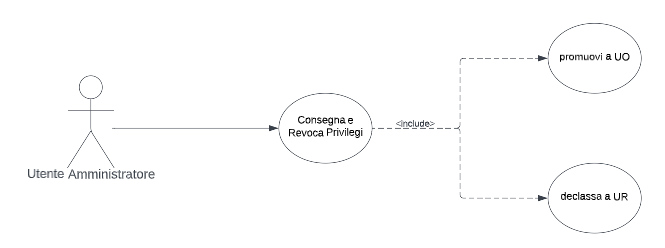
\includegraphics[scale=0.5]{UseCase_5.png}
\end{center}
\subsubsection*{Descrizione Use Case "Consegna e Revoca Privilegi"}
\begin{description}
    \item[] Titolo: Consegna e Revoca Privilegi
    \item[] Riassunto: Questo Use Case descrive come avviene la procedura di consegna e revoca privilegi
    \item[] Descrizione:
        \begin{enumerate}
            \item L'utente UA nella schermata "Impostazioni" seleziona l'opzione "Gestisci Privilegi"
            \item Il sistema presenta una schermata contenente un form in cui bisogna:
                  \begin{itemize}
                      \item Inserire la mail dell'utente da gestire
                      \item Selezionare il privilegio da assegnare
                  \end{itemize}
                  inoltre il sistema deve controllare l'\hyperref[exc:15.1]{[exception 1]}
        \end{enumerate}
    \item[] Exceptions:
        \begin{description}
            \item[] \label{exc:15.1} [exception 1] Tutti i campi devono essere compilati
        \end{description}
\end{description}
\renewcommand\thesubsection{\origthesubsection}
\clearpage
\section{Requisiti Non Funzionali}
\renewcommand\thesubsection{}
\subsection{RNF1 Privacy}
\begin{center}
    \begin{longtable}{|p{4cm}|p{8cm}|p{4cm}|}
        \hline
        Proprietà                                     & Descrizione                                                                                                                                                                                                                                                                                                                                                                                                                                                            & Misura   \\
        \hline
        Codice della Privacy                          & Per codice dalla privacy intendiamo la norma della Repubblica Italiana, emanata con il Decreto legislativo 30 giugno 2003, n. 196, in vigore dal 1º gennaio 2004.                                                                                                                                                                                                                                                                                                      & Conforme \\
        \hline
        Regolamento per la protezione dei dati (GDPR) & Il Regolamento Generale sulla Protezione dei Dati in sigla RGPD (o GDPR in inglese General Data Protection Regulation), ufficialmente regolamento (UE) n. 2016/679, è un regolamento dell'Unione europea in materia di trattamento dei dati personali e di privacy, adottato il 27 aprile 2016, pubblicato sulla Gazzetta ufficiale dell'Unione europea il 4 maggio 2016 ed entrato in vigore il 24 maggio dello stesso anno e operativo a partire dal 25 maggio 2018. & Conforme \\
        \hline
    \end{longtable}
\end{center}
\subsection{RNF2 Sicurezza}
\begin{center}
    \begin{longtable}{|p{4cm}|p{8cm}|p{4cm}|}
        \hline
        Proprietà                        & Descrizione                                                                          & Misura                          \\
        \hline
        Trasmissione dati autenticazione & Modalità di trasmissione delle credenziali raccolte in fase di autenticazione        & Utilizzo protocollo HTTPS       \\
        \hline
        Raccolta dati tramite form       & Modalità di trasmissione dei dati raccolti tramite i form proposti dall'applicazione & Utilizzo protocollo HTTPS       \\
        \hline
        Richiesta dati all'API           & Modalità di autorizzazione RestAPI                                                   & Utilizzo JWT e protocollo HTTPS \\
        \hline
    \end{longtable}
\end{center}
\subsection{RNF3 Scalabilità}
\begin{center}
    \begin{longtable}{|p{4cm}|p{8cm}|p{4cm}|}
        \hline
        Proprietà                                            & Descrizione                                                                 & Misura                                    \\
        \hline
        Elaborazione con un numero crescente di utenti       & Capacità del sistema di gestire un numero crescente di utenti in simultanea & Garantita fino a 100 utenti in simultanea \\
        \hline
        Memorizzazione dei dati con un numero alto di utenti & Capacità del sistema di gestire i dati generati da un alto numero di utenti & Garantita fino a 100 utenti               \\
        \hline
    \end{longtable}
\end{center}
\subsection{RNF4 Affidabilità}
\begin{center}
    \begin{longtable}{|p{4cm}|p{8cm}|p{4cm}|}
        \hline
        Proprietà          & Descrizione                                                                                          & Misura                        \\
        \hline
        Integrità dei dati & Per integrità dei dati si intende il mantenimento dei dati nel DataBase anche dopo dei guasti/errori & Creazione di Backup periodici \\
        \hline
    \end{longtable}
\end{center}
\subsection{RNF5 Memorizzazione}
\begin{center}
    \begin{longtable}{|p{4cm}|p{8cm}|p{4cm}|}
        \hline
        Proprietà & Descrizione                                                                                                        & Misura                     \\
        \hline
        TBD       & La memorizzazione dei dati avviene interamente su DataBase sul server quindi all'utente non verrà occupata memoria & Utilizzo di DataBase NoSQL \\
        \hline
    \end{longtable}
\end{center}
\subsection{RNF6 Compatibilità e Accessibilità}
\begin{center}
    \begin{longtable}{|p{4cm}|p{8cm}|p{4cm}|}
        \hline
        Proprietà                 & Descrizione                                                                             & Misura                                                                                 \\
        \hline
        Compatibilità con Android & Sistema operativo e versione a partire dalla quale l'applicazione può essere installata & L'applicazione deve essere compatibile con Android 8.0 o superiori                     \\
        \hline
        Compatibilità con iOS     & Sistema operativo e versione a partire dalla quale l'applicazione può essere installata & L'applicazione deve essere compatibile con iOS 12 o superiori                          \\
        \hline
        Compatibilità con Browser & Sistema operativo e versione a partire dalla quale l'applicazione può essere installata & L'applicazione deve essere compatibile con i principali browser: Firefox, Chrome, Edge \\
        \hline
    \end{longtable}
\end{center}
\subsection{RNF7 Supportabilità}
\begin{center}
    \begin{longtable}{|p{4cm}|p{8cm}|p{4cm}|}
        \hline
        Proprietà      & Descrizione               & Misura                                                                            \\
        \hline
        App supportate & Disponibilità di utilizzo & Sistema composto da web-app creato in React, quindi è disponibile su ogni browser \\
        \hline
    \end{longtable}
\end{center}
\subsection{RNF8 Facilità di Utilizzo}
\begin{center}
    \begin{longtable}{|p{4cm}|p{8cm}|p{4cm}|}
        \hline
        Proprietà         & Descrizione                                              & Misura                                                                                     \\
        \hline
        Accessibilità     & La mappa è scalabile                                     & L'utente può ingrandire la mappa a piacimento usando pulsanti appositi di zoom-in zoom-out \\
        \hline
        Personalizzazione & L'utente può personalizzare l'aspetto dell'app           & L'utente può cambiare tra light mode e dark mode all'interno delle impostazioni            \\
        \hline
        UI intuitiva      & L'utente può spostarsi tra le schermate in modo semplice & L'utente può spostarsi tra le schermate in modo semplice e intuitivo                       \\
        \hline
    \end{longtable}
\end{center}
\renewcommand\thesubsection{\origthesubsection}
\clearpage
\section{Analisi del Contesto}
\begin{description}
    \item[] Nel presente capitolo viene discusso il contesto del funzionamento del sistema
\end{description}
\subsection{Utenti e sistemi esterni}
\subsubsection{Utente}
\begin{description}
    \item[] Persona che utilizza il sistema per visualizzare gli eventi
\end{description}
\subsubsection{Utente Organizzatore}
\begin{description}
    \item[] Persona che utilizza il sistema per gestire (creazione, modifica ed eliminazione) gli eventi
\end{description}
\subsubsection{Utente Admin}
\begin{description}
    \item[] Utente amministratore ha il compito di gestire l'applicazione gestendo i vari eventi (creazione, modifica, eliminazione) e assegnando e revocando i privilegi agli utenti per trasformare un utente in utente organizzatore e viceversa
\end{description}
\subsubsection{DataBase}
\begin{description}
    \item[] Sistema usato per memorizzare i dati: utenti ed eventi
\end{description}
\subsection{Diagramma di Contesto}
\begin{description}
    \item[] 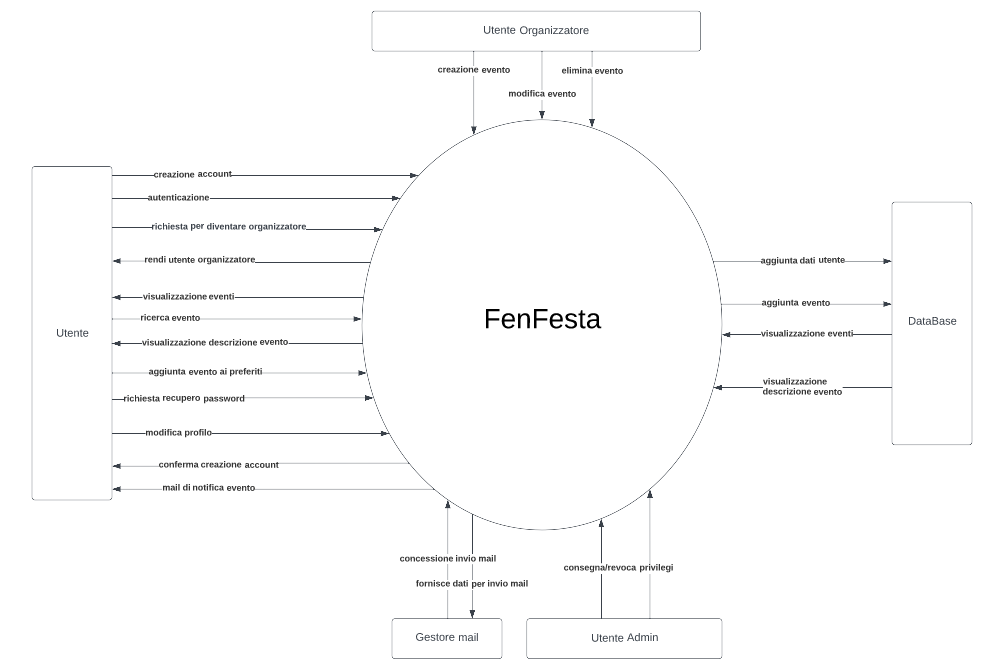
\includegraphics[scale=0.5]{Context.png} \\
        \textbf{Figura 1. Diagramma di Contesto per l'applicazione FenFesta} \label{fig:1}
    \item[] La \hyperref[fig:1]{Figura 1} mostra le principali interazioni tra attori o sistemi esterni e l'applicazione
\end{description}
\clearpage
\section{Analisi dei Componenti}
\begin{description}
    \item[] In questo capitolo viene descritta l'architettura dei componenti interni al sistema. \\
        Viene poi utilizzato il Component Diagram per rappresentare l'interconnessione tra i vari componenti
\end{description}
\subsection{Definizione dei componenti}
\begin{description}
    \item[] In questa sezione vengono definiti i vari componenti
\end{description}
\subsubsection{Creazione Account}
\begin{description}
    \item[] \underline{Motivazione:}
        Dati i requisiti per compiere alcune operazioni è necessario possedere un account.
\end{description}
\subsubsection{Gestore Autenticazione}
\begin{description}
    \item[] \underline{Motivazione:} Dati i requisiti l'autenticazione avviene tramite un sistema di credenziali interno. \\
\end{description}
\subsubsection{Gestore Account}
\begin{description}
    \item[] \underline{Motivazione:}
        Dati i requisiti è stata identificata la necessità di definire il componente \textbf{Gestore Account} per permettere all'utente di apportare modifiche al proprio account, di eliminare l'account, di richiedere l'upgrade dell'account, di recuperare la password.
\end{description}
\subsubsection{Gestore Notifiche}
\begin{description}
    \item[] \underline{Motivazione:}
        Necessitando, in linea con i requisiti, di un sistema per inviare comunicazioni con l'utenza è stato individuato il componente \textbf{Gestore Notifiche}.
\end{description}
\subsubsection{Creazione Evento}
\begin{description}
    \item[] \underline{Motivazione:}
        Il componente \textbf{Creazione Evento} è stato individuato per far fronte alla necessità dell'app di permettere la creazione di nuovi eventi da parte degli utenti con l'autorizzazione necessaria, in linea con le specifiche dei requisiti.
\end{description}
\subsubsection{Gestore Eventi}
\begin{description}
    \item[] \underline{Motivazione:} Dati i requisiti, si individua il componente \textbf{Gestore Eventi} per modificare ed eliminare gli eventi nel database e per inoltrare i dati agli altri componenti.
\end{description}
\subsubsection{Mappa}
\begin{description}
    \item[] \underline{Motivazione:}
        Come da requisiti è necessario il componente \textbf{Mappa}, il quale si occupa di presentare gli eventi distribuendoli su una mappa.
\end{description}
\subsubsection{Elenco Eventi}
\begin{description}
    \item[] \underline{Motivazione:}
        Dati i requisiti è stata identificata la necessità di definire il componente \textbf{Elenco Eventi}, il quale si occupa di presentare all' utente gli eventi in un elenco
\end{description}
\subsubsection{Gestore Visualizzazione Evento}
\begin{description}
    \item[] \underline{Motivazione:}
        Dati i requisiti è stata identificata la necessità di definire il componente \textbf{Gestore Visualizzazione Evento}, il quale mostra all'utente informazioni riguardanti ul singolo evento e permette di di segnalare la propria partecipazione e/o aggiungere ai preferiti l'evento
\end{description}
\subsubsection{Gestore Preferiti}
\begin{description}
    \item[] \underline{Motivazione:}
        Dati i requisiti è stata identificata la necessità di definire il componente \textbf{Gestore Preferiti}, il quale si occupa di aggiungere ai preferiti dell'utente l'evento precedentemente visualizzato.
\end{description}
\clearpage
\subsection{Diagramma dei componenti}
\begin{description}
    \item[] 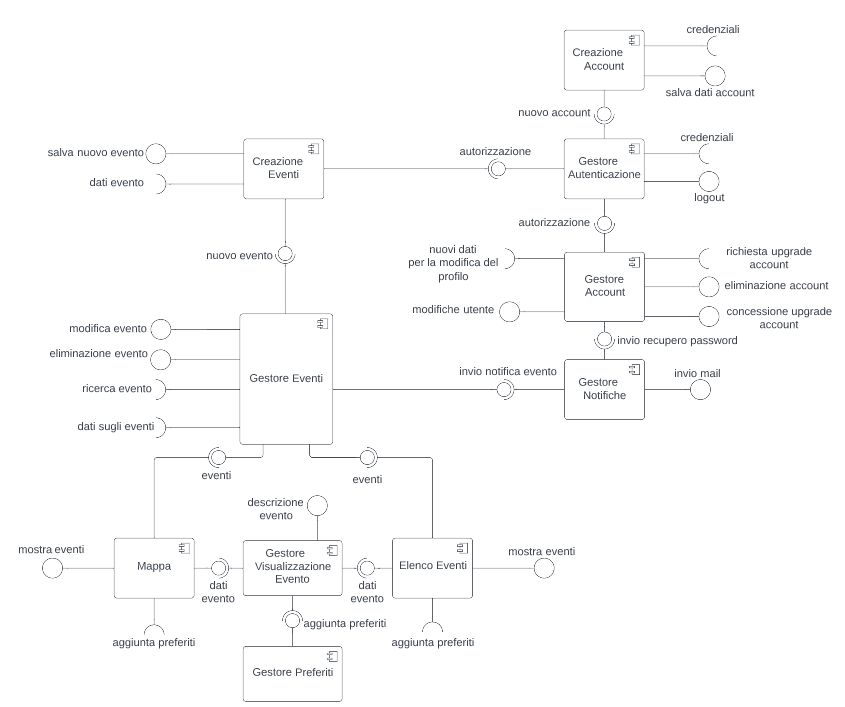
\includegraphics[scale=0.6]{Component.png} \\
        \textbf{Figura 2. Diagramma dei Componenti per l'applicazione FenFesta} \label{fig:2}
\end{description}
\subsubsection{Creazione Account}
\begin{description}
    \item[] \underline{Descrizione:} Il componente \textbf{Creazione Account} si occupa di permettere all'utente di creare un proprio account unico andandolo a salvare nel database dell'app.
    \item[] \underline{Interfaccia Richiesta - Credenziali:} Le credenziali richieste alla registrazione includono email, password e conferma della password
    \item[] \underline{Interfaccia Fornita - Salva dati account:} Al momento della creazione di un nuovo account esso viene fornito al \textbf{Database} per l'imagazzinamento di esso
    \item[] \underline{Interfaccia Fornita - Nuovo account:} Al momento della creazione di un nuovo accout esso viene fornito al \textbf{Gestore Autenticazione}
\end{description}
\subsubsection{Gestore Autenticazione}
\begin{description}
    \item[] \underline{Descrizione:} Il componente \textbf{Gestione Autenticazione} gestirà tutte le operazioni di autenticazione mantenendo poi attiva la sessione dell'utente nell'applicazione.
    \item[] \underline{Interfaccia Richiesta - Credenziali:} Le credenziali richieste al login includono email, password
    \item[] \underline{Interfaccia Richiesta - Nuovo account:} Il gestore richiede accesso agli account creati dal componente \textbf{Creazione Account} per verificare le credenziali
    \item[] \underline{Interfaccia Fornita - Autorizzazione:} Una volta effettuato il login il \textbf{Gestore Autenticazione} fornisce agli altri componenti la sessione dell'utente
\end{description}
\subsubsection{Gestore Account}
\begin{description}
    \item[] \underline{Descrizione:} Permette all'utente di apportare modifiche al proprio account in base ai privilegi di cui si dispone (modifica password per account base, modifica dati organizzatore per account organizzatore), di eliminare l'account, di richiedere l'upgrade dell'account (mentre sempre grazie a questo componente l'admin può elargire tali upgrade), di recuperare la password (comunicando la necessità di un invio mail al componente \textbf{Gestore Notifiche})
    \item[] \underline{Interfaccia Richiesta - Autorizzazione:} Sessione utente fornita dal \textbf{Gestore Autenticazione}
    \item[] \underline{Interfaccia Richiesta - Dati modifica profilo:} Dati modificati dall'utente richiesti per effettuare la modifica del proprio profilo
    \item[] \underline{Interfaccia Richiesta - Richiesta upgrade account:} Richiesta per effettuare l'upgrade da utente registrato \textbf{UR} a utente organizzatore \textbf{UO}
    \item[] \underline{Interfaccia Fornita - Eliminazione account:} Dati riguardanti l'eliminazione del profilo diretti al \textbf{Database}
    \item[] \underline{Interfaccia Fornita - Modifica account:} Dati riguardanti la modifica del profilo diretti al \textbf{Database}
    \item[] \underline{Interfaccia Fornita - Concessione upgrade account:} Concessione fornita da un utente admin \textbf{UA} verso un utente registrato \textbf{UR} per effettuare l'upgrade del proprio account
    \item[] \underline{Interfaccia Fornita - Invio recupero password:} Una volta effettuata la richiesta di recupero password il componente invia al \textbf{Gestore Notifiche} i dati per successivamente creare e mandare la mail all'utente
\end{description}
\subsubsection{Gestore Notifiche}
\begin{description}
    \item[] \underline{Descrizione:} Il componente si interfaccerà con un sistema esterno per l'invio di mail riguardanti gli eventi prossimi e le eventuali richieste di recupero password.
    \item[] \underline{Interfaccia Richiesta - Invio recupero password:} Dati ricevuti dal \textbf{Gestore Account} per successivamente inviare una mail all'utente, contenente il recupero delle credenziali
    \item[] \underline{Interfaccia Richiesta - Invio notifica evento:} Dati richiesti per successivamente mandare la notifica all'utente riguardante gli eventi da esso preferiti
    \item[] \underline{Interfaccia Fornita - Invio Mail:} Dati forniti al \textbf{Gestore Mail} per inviare le mail
\end{description}
\subsubsection{Creazione Evento}
\begin{description}
    \item[] \underline{Descrizione:} Il componente permette ad un utente autorizzato di creare nuovi eventi. Una volta ricevuti dall'utente i dati riguardo il nuovo evento da aggiungere al database, il componente, verificata la validità delle informazioni inserite, aggiungerà il nuovo evento al database per permettere ad altri componenti di interfacciarsi con suddetti dati.
    \item[] \underline{Interfaccia Richiesta - Autorizzazione:} Sessione utente fornita dal \textbf{Gestore Autenticazione}
    \item[] \underline{Interfaccia Richiesta - Dati evento:} Dati richiesti all'utente organizzatore \textbf{UO} per la creazione di un nuovo evento
    \item[] \underline{Interfaccia Fornita - Nuovo evento:} Al momento della creazione di un nuovo evento esso viene fornito al \textbf{Gestore Eventi}
    \item[] \underline{Interfaccia Fornita - Salva nuovo evento:} una volta creato l'evento il componente invia i dati al \textbf{Database}
\end{description}
\subsubsection{Gestore Eventi}
\begin{description}
    \item[] \underline{Descrizione:} Il componente permetterà agli utenti autorizzati (proprietario e admin) di apportare modifiche ed eliminare gli eventi presenti nel database. Inoltre fornisce i dati (i vari eventi presenti in database) necessari ai componenti \textbf{Mappa} e \textbf{Elenco Eventi}, filtrandoli se necessario in base alla stringa di ricerca scelta dall'utente. Si occupa di inviare richieste di invio notifica al componente \textbf{Gestore Notifiche}.
    \item[] \underline{Interfaccia Richiesta - Nuovo evento:} Il gestore richiede accesso ai nuovi eventi creati dal componente \textbf{Creazione Evento} per verificarne i dati
    \item[] \underline{Interfaccia Richiesta - Ricerca evento:} Dati richiesti riguardanti la ricerca di un evento specifico
    \item[] \underline{Interfaccia Richiesta - Dati evento:} Dati richiesti all'utente organizzatore \textbf{UO} per la modifica di un evento
    \item[] \underline{Interfaccia Fornita - Modifica evento:} Dati riguardanti alla modifica di un evento forniti al \textbf{Database}
    \item[] \underline{Interfaccia Fornita - Eliminazione evento:} Dati riguardanti l'eliminazione di un evento forniti al \textbf{Database}
    \item[] \underline{Interfaccia Fornita - Lista eventi:} Dati riguardanti la lista degli eventi forniti ai componenti \textbf{Mappa} e \textbf{Elenco eventi}
\end{description}
\subsubsection{Mappa}
\begin{description}
    \item[] \underline{Descrizione:} Coerentemente con i dati geografici presenti nei dati evento ricevuti dal componente \textbf{Gestore Eventi}, il componente renderizza una mappa con l'ausilio di un servizio esterno. Selezionando un evento si passa alla visualizzazione delle sue informazioni, gestita dal componente \textbf{Gestione Visualizzazione Evento}.
    \item[] \underline{Interfaccia Richiesta - Lista eventi:} Lista degli eventi da mostrare all'utente
    \item[] \underline{Interfaccia Fornita - Mostra eventi:} Dati riguardanti gli eventi, sono forniti all'utente sotto forma di visualizzazione
    \item[] \underline{Interfaccia Fornita - Dati evento:} Dati dell'evento specifico forniti al \textbf{Gestore Visualizzazione Evento} per visualizzarne i dettagli
\end{description}
\subsubsection{Elenco Eventi}
\begin{description}
    \item[] \underline{Descrizione:} Il componente si occupa di presentare all' utente gli eventi in un elenco. Selezionando un evento si passa alla visualizzazione delle sue informazioni, gestita dal componente \textbf{Gestione Visualizzazione Evento}
    \item[] \underline{Interfaccia Richiesta - Lista eventi:} Lista degli eventi da mostrare all'utente
    \item[] \underline{Interfaccia Fornita - Mostra eventi:} Dati riguardanti gli eventi, sono forniti all'utente sotto forma di visualizzazione
    \item[] \underline{Interfaccia Fornita - Dati evento:} Dati dell'evento specifico forniti al \textbf{Gestore Visualizzazione Evento} per visualizzarne i dettagli
\end{description}
\subsubsection{Gestore Visualizzazione Evento}
\begin{description}
    \item[] \underline{Descrizione:} Permette di visualizzare informazioni sul singolo evento selezionato o dal componente \textbf{Mappa} o dal componente \textbf{Elenco Eventi}. Permette inoltre di richiedere di aggiungere un evento ai preferiti dell'utente, richiesta che verrà presa in carico dal componente \textbf{Gestore Preferiti}. L'utente può segnalare la propria partecipazione
    \item[] \underline{Interfaccia Richiesta - Dati evento:} Dati dell'evento specifico richiesti sia dal componente \textbf{Mappa} che dal componente \textbf{Elenco Eventi}
    \item[] \underline{Interfaccia Richiesta - Segnalazione partecipazione:} Dato riguardante la partecipazione di un utente ad un evento forniti al \textbf{Gestore Visualizzazione Evento} stesso
    \item[] \underline{Interfaccia Richiesta - Aggiunta preferiti:} Dati riguardanti la preferenza di un evento per un utente persi in input dall'utente stesso
    \item[] \underline{Interfaccia Fornita - Aggiunta preferiti:} Dati riguardanti la preferenza di un evento per un utente forniti al componente \textbf{Gestore Preferiti}
    \item[] \underline{Interfaccia Fornita - Descrizione evento:} Dati forniti all'utente riguardanti la descrizione del evento precedentemente selezionato
\end{description}
\subsubsection{Gestore Preferiti}
\begin{description}
    \item[] \underline{Descrizione:} Il componente si occupa di aggiungere ai preferiti dell'utente l'evento visualizzato nel componente \textbf{Gestore Visualizzazione Evento}, gli eventi prossimi vengono segnalati al componente \textbf{Gestore Notifiche}
    \item[] \underline{Interfaccia Richiesta - Aggiunta Preferiti:} Dati richiesti al \textbf{Gestore Visualizzazione Evento} riguardo l'evento da aggiungere ai preferiti dell'utente
    \item[] \underline{Interfaccia Fornita - Invio Notifica Evento:} Fornisce al componente \textbf{Gestore Notifiche} i dati relativi all'evento prossimo per permettere la generazione di una notifica
    \item[] \underline{Interfaccia Fornita - Salva preferito:} Dati forniti al \textbf{Database} per salvare l'evento come preferito
\end{description}
\end{document}